\subsection{Results}
The analysed architectures are mainly two, one in which all the blocks have been described from a behavioural point of view and the other in which it has been chosen how to synthesise some more critical combinatorial blocks. The behavioural description allows the Synopsys synthesis tool to perform all optimisations and to choose the best structure based on the given constraints. On the other hand, when choosing a particular structure Synopsys is constrained to use it, and sometimes better results can be achieved.\\
In the case analysed hereafter, for example, a summator implemented as a Carry-Save-Adder was chosen with regard to the ALU in the constrained version.\\
The performance analysis was repeated twice, once for the first implementation of the RISC-V processor and again for the processor with the ISA modified by the addition of the absolute value instruction. In the \autoref{tab:results} it can be seen, as expected, that the optimisations performed by Synopsys when fewer constraints are present are more effective, both in the base case and with the modified ISA.\\
\begin{table}[H]
	\centering
	\begin{tabular}{c|c|c||c|c}
		& Base model & CSA & Base ABS & ABS  \& CSA \\
		\hline
		Clock frequency (ns) & 1.26 & 1.33 & 1.30 & 1.38 \\
		Comb. Area ($\mu m^2$) & 6430 & 6975 & 6909 & 7242 \\
		Non Comb. Area ($\mu m^2$) & 6471 & 6459 & 6469 & 6462 \\
		Total Area ($\mu m^2$)	& 12902 & 13435 & 13378 & 13705 \\
	\end{tabular}
	\caption{Results of the synthesis}
	\label{tab:results}
\end{table}

\noindent From an area perspective, the main differences between the four analyzed cases concern the occupation of the combinational part of the circuit. In particular, it can be seen that in both cases the area increases by 5\% when the implementation of the adder is done with the CSA and that by inserting the absolute value module inside the ALU the area increases by a further 10\%.
The area of the non-combinational part, on the other hand, remains more or less constant in all cases since the major changes are in the combinational blocks. In terms of total area, therefore, the differences between the various implementations are halved, having the two contributions a very similar value.\\
Both after extracting the netlist and after running the place \& route, the DUT was simulated with the input vectors used in the \autoref{sec:test}, and the results were identical to the previous ones. 

\begin{figure}[H]
	\centering
	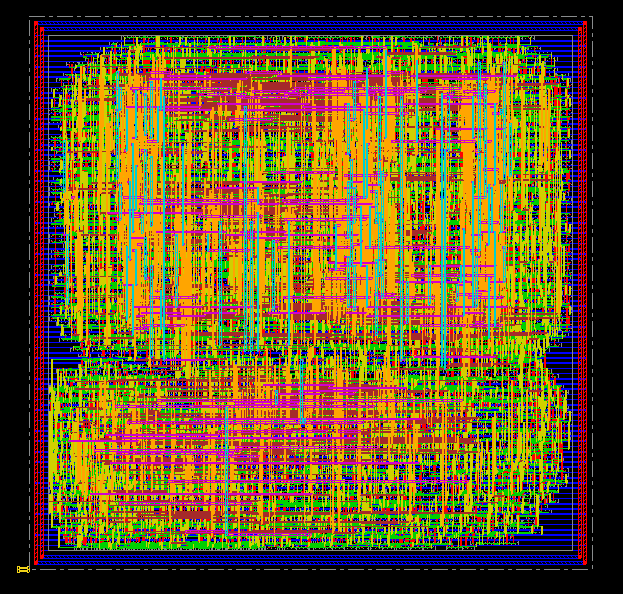
\includegraphics[width=0.5\textwidth]{sec4/images/place.png}
	\caption{Layout after place phase}
	\label{fig:place}
\end{figure}

\begin{figure}[H]
	\centering
	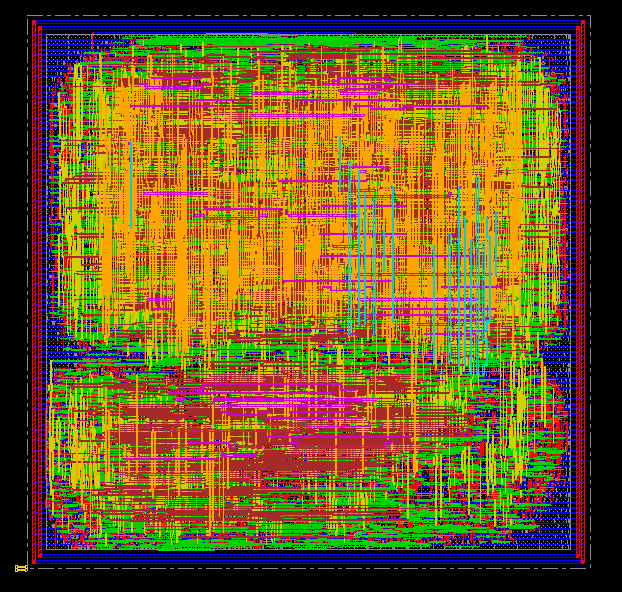
\includegraphics[width=0.5\textwidth]{sec4/images/route.png}
	\caption{Layout after place\&route}
	\label{fig:route}
\end{figure}